\documentclass[a4paper,10pt,twoside]{article}
\pdfoutput=1 

\usepackage{amssymb,amsmath}       % Equations
\usepackage{array}
\usepackage{bm}                    % Bold math symbols
\usepackage{epsfig}
\usepackage{float}
\usepackage{graphicx,color,psfrag} % Graphics, Figures
\usepackage[export]{adjustbox}
\usepackage{subcaption}
\usepackage{tikz}
% \graphicspath{ {Users/Simba/Documents/Academic\ Info/PhD/courses/algorithm/images} }
\usepackage{multirow}              % For Tables
\usepackage{tabularx}              % Tables
\usepackage{wrapfig}
\usepackage[algoruled]{algorithm2e}
\SetStartEndCondition{ }{}{}%
\SetKwProg{Fn}{def}{\string:}{}
\SetKwFunction{Range}{range}%%
\SetKw{KwTo}{in}\SetKwFor{For}{for}{\string:}{}%
\SetKwIF{If}{ElseIf}{Else}{if}{:}{elif}{else:}{}%
\SetKwFor{While}{while}{:}{}%
% \renewcommand{\forcond}{$i$ \KwTo\Range{$n$}}
\AlgoDontDisplayBlockMarkers\SetAlgoNoEnd\SetAlgoNoLine%


%% enumitem 
% \labelindent is defined in both IEEEtrans and
% enumitem. \let\labelindent\relax kind-of disables \labelindent
% defined in IEEEtrans, hence avoiding the name clash.
\let\labelindent\relax
\usepackage[inline]{enumitem}

%% algorithm2e
% \usepackage[plain]{algorithm2e}
% remove line number for one line
% \let\oldnl\nl
% \newcommand{\nonl}{\renewcommand{\nl}{\let\nl\oldnl}}

%% subfigure
\usepackage[caption=false,font=footnotesize]{subfig}
% make references to subfigures appear as \thefigure(\thesubfigure)
\captionsetup[subfigure]{subrefformat=simple,labelformat=simple,listofformat=subsimple}
\renewcommand\thesubfigure{(\alph{subfigure})}

% variables
\newcommand{\mc}[2][]{{\mathcal{#2}_{\textrm{#1}}}}
\newcommand{\q}[1]{\bm{q}_{\textrm{#1}}}
\newcommand{\qd}[1]{\bm{\dot{q}}_{\textrm{#1}}}
\newcommand{\T}[1]{\bm{T}_{\textrm{#1}}}
\newcommand{\x}[1]{\bm{x}_{\textrm{#1}}}
\newcommand{\qvect}{\bm{q}}
\newcommand{\Tvect}{\bm{T}}
\newcommand{\GP}{\mathcal{G}\cap\mathcal{P}}
\newcommand{\cP}{\mathcal{P}}
\newcommand{\cC}{\mathcal{C}}
\newcommand{\cO}{\mathcal{O}}
\newcommand{\bfp}{\mathbf{p}}
\newcommand{\calT}{\mathcal{T}}
\DeclareMathOperator*{\argmin}{arg\,min}
\DeclareMathOperator*{\argmax}{arg\,max}
% acronyms
\newcommand{\ie}{{\textit{i.e.}}}
\newcommand{\etal}{\textit{et~al.}}

% theorem environment
\newtheorem{theorem}{Theorem}
\newtheorem{proof}{Proof}
\newtheorem{lemma}{Lemma}
\newtheorem{proposition}{Proposition}
\newtheorem{corollary}{Corollary}
\newtheorem{remark}{Remark}
% TODO
\newcommand{\TODO}[1]{\noindent {\color{red} \{{\bf To-do:} #1\}}}
% COMMENT
\newcommand{\comment}[1]{}

% change tt font
\renewcommand{\tt}{\fontfamily{cmtt}\selectfont}

% figures path
\graphicspath{{figures/}}

% \overrideIEEEmargins
% set margins
\setlength{\floatsep}{2pt plus 1pt minus 1pt}
\setlength{\textfloatsep}{5pt plus 1pt minus 2pt}

%% TITLE
\title{MAS714-Homework 2}
%% AUTHOR
\author{Pham Tien Hung, Zhang Xu
}

%% DATE
\date{}


%%%%%%%%%%%%%%%%%%%%%%%%%%%%%%%%%%%%%%%%%%%%%%%%%%%%%%%%%%%%%%%%%%%%%%
\begin{document}
\maketitle
\section*{Excercise 1}
\subsection*{a)}
Prove that every tree is a bipartite graph.
\begin{proof}
	We will prove by induction, that is every tree $T(V, E)$ whose
	$|V| = n$ for all $n$ is a bipartite graph. The case $n=2$ is trivially true.

	Assume that this is true for $n = k$, we will now prove that it
	is true for $n = k + 1$. 

	Consider we add a leaf node $u$ to a tree $T$ with $|V| = k$, 
	if its parent belongs to $L$, then the node $u$ has to go to set $R$, vice versa. 
	Therefore it is true for $n = k + 1$.

	It is proven that every tree is a bipartite graph.
		
\end{proof}

\subsection*{b)}


	\TODO{}

\section*{Excercise 2}

Assume that $X_L[1...n]$ is sorted with $X_L[1]$ being the smallest member.

\begin{algorithm}[h]
\caption{Find maximum tiling ($X$):}
	Initialize $T = \emptyset$\;
	Let $x_{stop} = X_R[1]$;
	\While{$X$ is not empty}{
		Let $x_{max} = -\infty$\;
		\While{$X_L[1] \leq x_{stop}$}{
			\If {$X_R[1] > x_{max}$}{
				$x_{max} = X_R[1]$\;
				Select $X[1]$ as the chosen interval $i$\;
			}
			Remove $X[1]$ from $X$\;
		}
		Add the selected interval $i$ to $T$\;
		Let $x_{stop} = x_{max}$;
	}
	\Return $T$\;
\end{algorithm}
Running time $O(n)$.

\begin{proof}
	Feasibility: The algorithm chooses interval that has the largest right endpoint and overlaps with 		its preceding interval. Clearly it will return a tiling path.
	Optimality: Assume by contradiction that the greedy algorithm is not optimal.
	Let $i_{1}, i_{2}, . . . , i_{k}$ denote set of intervals selected by the algorithm.
	Let $j_{1}, j_{2}, . . . , j_{m}$ denote set of intervals in an optimal solution with 
	$i_{1} = j_{1}, i_{2} = j_{2}, . . . , i_{r} = j_{r}$ for the largest possible value of $r$.
	Replace interval $j_{r+1}$ with interval $i_{r+1}$. Since interval $i_{r+1}$ exists and has larger 			right endpoint than $j_{r+1}$, the new solution still feasible and optimal. 
	Thus maximality of $r$ is contradicted.

\end{proof}

\section*{Excercise 3}
\subsection*{a)}
Not every minimum bottleneck spanning tree (MBT) is a minimum spanning tree (MST).
Refer to the counterexample below. 
\begin{figure}[h]
 
\begin{subfigure}{0.3\textwidth}
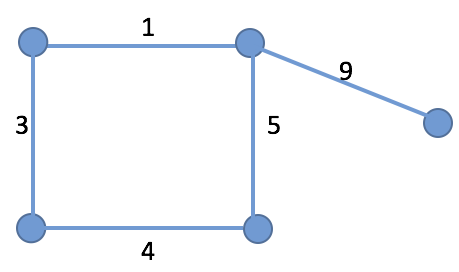
\includegraphics[width=0.9\linewidth, height=3cm]{G} 
\caption{G}
\label{fig:subim1}
\end{subfigure}
\begin{subfigure}{0.3\textwidth}
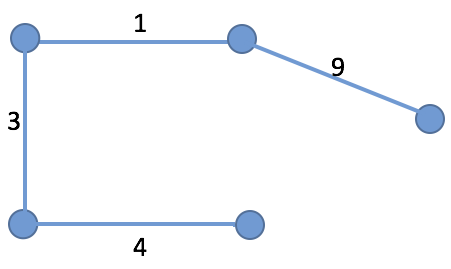
\includegraphics[width=0.9\linewidth, height=3cm]{MST}
\caption{MST}
\label{fig:subim2}
\end{subfigure}
 \begin{subfigure}{0.3\textwidth}
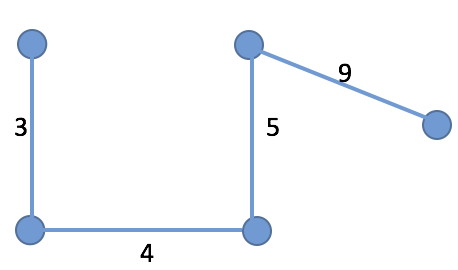
\includegraphics[width=0.9\linewidth, height=3cm]{MBST}
\caption{MBST}
\label{fig:subim3}
\end{subfigure}
\end{figure}

Take the connected graph G in (a) as an example. (b) presents its minimum spanning tree (MST) and (c) is one minimum-bottleneck spanning tree (MBST) of G, which is clearly different from MST. 

\subsection*{b)}
We will show that for an undirect graph $G$, a minimum spanning tree (MST) is a minimum-bottleneck spanning tree (MBST).
\begin{proof}
	Prove by contradition. 
	Assume $T$ is a MST for graph $G$ with the largest cost of edge to be $w(u, v) = a$,
	$T'$ is an MBST for graph $G$ with the largest cost of edge to be $w(u', v') = b < a$.
	Let $e(u, v)$ be the cut edge in MST that partitions all vertices into two sub trees 
	$T_{l}$ and $T_{r}$. By our assumption $e(u, v)$ is not in $T'$ as $w(u, v) = a > b$.
	If edge $e(i, j)$ with cost $c$ is in $T'$ to connect $T_{l}$ and $T_{r}$, according to definition 			of MBST, $c \leq b$. At the same time, by definition of MST, $c$ should be larger than $a$. 			These two conditions indicate that $a < b$, which contradits our assumption.

\end{proof}



\end{document}
